\documentclass[pdf]{beamer}
\mode<presentation>{}
\usetheme{Dresden}
\usepackage{apalike}
\usepackage{graphicx}
\usepackage{subcaption}
\usepackage{pgfplotstable}
\usepackage{graphicx,psfrag}
\usepackage{mwe,tikz}\usepackage[percent]{overpic}
%% preamble
\title{Behaviour of The Serre Equations In The Presence of Steep Gradients}
\author{Jordan Pitt, Stephen Roberts and Christopher Zoppou \\ Australian National University}
\newcommand\solidrule[1][0.25cm]{\rule[0.5ex]{#1}{1pt}}
\newcommand\dashedrule{\mbox{\solidrule[2mm]\hspace{2mm}\solidrule[2mm]}}
\newcommand{\dotrule}[1]{%
	\parbox[]{#1}{\dotfill}}

\begin{document}
%% title frame
\section{Introduction}
\begin{frame}
\titlepage
\end{frame}

\section{Problem}
\subsection{Introduction}
\begin{frame}{Problem}
Goal: numerically model a tsunami throughout its evolution efficiently and robustly.
\begin{itemize}
\pause
\item Numerically Model: want a numerical method for partial differential equations that model fluids
\pause
\item Tsunami
\pause
 : Tohoku 2011
\end{itemize}
\begin{figure}
	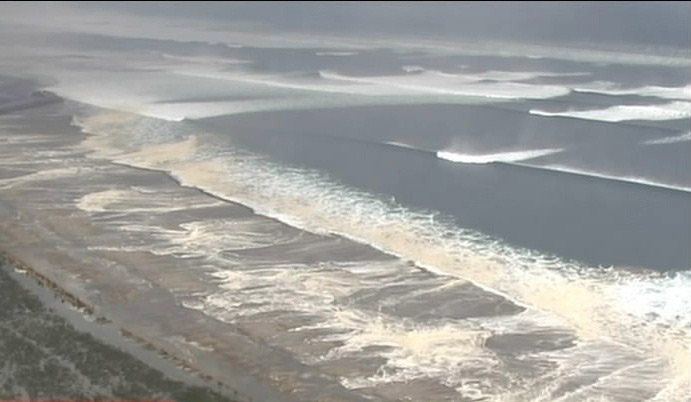
\includegraphics[width=0.55\textwidth]{../Pics/Web/1.jpg}
\end{figure}


%first let me give a brief overview of the main numerical method types, the tools we have to accomplish this task
\end{frame}

\begin{frame}{Problem}
	Goal: numerically model a tsunami throughout its evolution efficiently and robustly.
	\begin{itemize}
		\item Numerically Model: want a numerical method for partial differential equations that model fluids
		\item Tsunami
		\item Efficiently: our method must not be too computationally demanding
		\pause
		\item Robustly: our method should handle all types of initial conditions and situations that arise from them, the main difficulty usually is the presence of steep gradients. 
	\end{itemize}
	
	%first let me give a brief overview of the main numerical method types, the tools we have to accomplish this task
\end{frame}



\begin{frame}{Problem}
Goal: numerically model a tsunami throughout its evolution efficiently and robustly.
\vskip 0.2cm
Step 1: Pick partial differential equations that model tsunamis well and have robust and efficient methods. We focus on two dimensional flow first.

%first let me give a brief overview of the main numerical method types, the tools we have to accomplish this task
\end{frame}

\subsection{Partial Differential Equations}
\begin{frame}{PDEs}
Non-exhaustive list of PDES that describe fluid dynamics well for tsunamis from most difficult to solve to easiest
\begin{itemize}
\item Navier-Stokes equations
\item inviscid incompressible Euler equations
\item Serre equations
\item shallow water wave equations
\end{itemize}
\end{frame}

\begin{frame}{Navier-Stokes / Euler Equations}
Coordinates: ($x$,$z$) over time $t$

Function of $\rho$ (density), $\mathbf{u} = (u,w)$ (velocity), $p$ (pressure)

 , $\boldsymbol{\tau}$ (stress tensor) and $\mathbf{g}$ (acceleration due to gravity)
\vskip 0.2cm
Conservation of mass:	
\[\frac{\partial \rho}{\partial t} +  \nabla \cdot \left(\rho \mathbf{u}\right) = 0\]

Conservation of momentum:
\[ \frac{\partial \left(\rho\mathbf{u} \right)}{\partial t} + \nabla \cdot \left(\rho \mathbf{u} \times \mathbf{u}^T  \right) =  - \nabla\cdot p \mathbf{I} + \nabla \cdot \boldsymbol{\tau} + \rho \mathbf{g}\]

\end{frame}

\begin{frame}{Navier-Stokes / Euler Equations}
		
\begin{enumerate}
	\item Models fluids in the general case very well
	\pause
	\item Can neglect stress tensor and density differences for tsunamis (inviscid incompressible Euler Equations)
	\pause
	\item No methods that are efficient and robust for our domains of interest
	\pause
	\item No analytic solutions for problems containing steep gradients
\end{enumerate}
\end{frame}

\begin{frame}{Shallow Water Wave Equations}
Coordinates are ($x$,$z$) over time $t$ \\
$h(x,t)$: water depth \\
$\mathbf{u} = (u,w)$: velocities over water depth \\
$g$: acceleration due to gravity\\
assumption that $w = 0$. 
	\begin{subequations}
		Conservation of mass:
		\begin{gather*}
		\dfrac{\partial h}{\partial t} + \dfrac{\partial (uh)}{\partial x} = 0,
		\end{gather*}
		Conservation of momentum:
		\begin{gather*}
		\dfrac{\partial (uh)}{\partial t} + \dfrac{\partial}{\partial x} \left ( u^2h + \dfrac{gh^2}{2}\right ) = 0 
		\end{gather*}
	\end{subequations}

\end{frame}

\begin{frame}{Shallow Water Wave Equations}
	
\begin{enumerate}
	\pause
	\item Free surface approximation
	\pause
	\item No vertical motion of fluid
	\pause
	\item Models tsunamis well, but does not capture all behaviour (dispersion)
	\pause
	\item Efficient and robust methods
	\pause
	\item Analytic solutions for problems containing steep gradients
\end{enumerate}
\end{frame}

\begin{frame}{Compromise: Serre Equations}
Coordinates are ($x$,$z$) over time $t$ \\
$h(x,t)$: water depth \\
$\mathbf{u} = (u,w)$: velocities over water depth \\
$g$: acceleration due to gravity\\
assumption that $w = -z \frac{\partial u}{\partial x}$. 
	
	\begin{subequations}
		Conservation of mass:
		\begin{gather*}
		\dfrac{\partial h}{\partial t} + \dfrac{\partial (uh)}{\partial x} = 0,
		\end{gather*}
		Conservation of momentum:
		\begin{gather*}
		\underbrace{\underbrace{\dfrac{\partial (uh)}{\partial t} + \dfrac{\partial}{\partial x} \left ( u^2h + \dfrac{gh^2}{2}\right )}_{\text{Shallow Water Wave Equations}} + \underbrace{\dfrac{\partial}{\partial x} \left (  \dfrac{h^3}{3} \left [ \dfrac{\partial u }{\partial x} \dfrac{\partial u}{\partial x} -u \dfrac{\partial^2 u}{\partial x^2}  - \dfrac{\partial^2 u}{\partial x \partial t}\right ] \right )}_{\text{Dispersion Terms}} = 0}_{\text{Serre Equations}}
		\end{gather*}
	\end{subequations}
	
	
\end{frame}

\begin{frame}{Compromise: Serre Equations}
\begin{enumerate}
	\pause
	\item Free surface approximation
	\pause
	\item Vertical velocity of fluid is linear across depth
	\pause
	\item Captures more behaviour than the shallow water wave equations such as dispersion
	\pause
	\item Efficient and robust methods
	\pause
	\item Cannot model wave breaking 
\end{enumerate}	
\end{frame}

\begin{frame}{Problem}
Goal: Numerically model a tsunami throughout its evolution efficiently and robustly.
\vskip 0.2cm
Step 1: We choose the Serre equations as a compromise between the shallow water wave equations and the Navier-Stokes/ Euler equations
\vskip 0.2cm
New Problem: Efficient numerical method

\end{frame}

\section{Numerical Methods}
\begin{frame}
	3 Main Types of Numerical Methods
	\begin{itemize}
		\item Finite Difference
		\item Finite Element
		\item Finite Volume
	\end{itemize}
\end{frame}

\subsection{Finite Difference}
\begin{frame}{Finite Difference}
	We approximate derivatives at a point $x_0$ using function evaluations at nearby points, for example
	\[f'(x_0) \approx \frac{f(x_0+\Delta x) - f(x_0)}{\Delta x}\]
	
	The accuracy of this approximation depends on both $f$ and $\Delta x$, although we focus on $\Delta x$.
\end{frame}
\begin{frame}{Main Tool Taylor Series}
	Provided $f$ infinitely differentiable around $x_0$
	\[ f(x) = f(x_0) + \frac{f'(x_0)}{1!}(x - x_0) + \frac{f''(x_0)}{2!}(x - x_0)^2 + \dots\]
	\pause
	\[ f(x_0 + \Delta x) = f(x_0) + f'(x_0)\Delta x + \frac{f''(x_0)}{2!}(\Delta x)^2 + \dots\]
\pause	
	\[ \frac{f(x_0 + \Delta x) - f(x_0)}{\Delta x} = f'(x_0) + \frac{f''(x_0)}{2!}(\Delta x) +   \dots\]
\pause
	\[  f'(x_0)  = \frac{f(x_0 + \Delta x) - f(x_0)}{\Delta x} - \frac{f''(x_0)}{2!}(\Delta x) -   \dots\]
	
\end{frame}
\begin{frame}{Application}
	Serre equations
	\begin{subequations}
		\begin{gather*}
		\dfrac{\partial h}{\partial t} + \dfrac{\partial (uh)}{\partial x} = 0,
		\end{gather*}
		\begin{gather*}
		\dfrac{\partial (uh)}{\partial t} + \dfrac{\partial}{\partial x} \left ( u^2h + \dfrac{gh^2}{2}\right )+ \dfrac{\partial}{\partial x} \left (  \dfrac{h^3}{3} \left [ \dfrac{\partial u }{\partial x} \dfrac{\partial u}{\partial x} -u \dfrac{\partial^2 u}{\partial x^2}  - \dfrac{\partial^2 u}{\partial x \partial t}\right ] \right )= 0
		\end{gather*}
	\end{subequations}
	
Expand all terms then approximate them as finite differences.
\end{frame}

\subsection{Finite Volume}

\begin{frame}{Finite Volume}
	Equation in conservative form
	\[\frac{\partial }{\partial t}u = - \frac{\partial }{\partial x}f(u) \]
	
	Spatial grid: $x_i$ uniform so that $\Delta x = x_i - x_{i-1}$ for all $i$
	\vskip 0.2cm
	Temporal grid: $t^n$ uniform so that $\Delta t = t^n - t^{n-1}$ for all $n$
	\vskip 0.2cm
	Cells: $i$th cell centred around $x_i$ is $\mathcal{C}_i = \left[x_i - \frac{\Delta x}{2},x_i + \frac{\Delta x}{2} \right]$
	
\end{frame}

\begin{frame}
	Integrating our PDE over $\mathcal{C}_i$ and time step gives

	\begin{multline*}
	\int_{\mathcal{C}_i}u(x,t^{n+1}) \;dx -\int_{\mathcal{C}_i}u(x,t^{n}) \;dx  \\=  \int_{t^n}^{t^{n+1}}f\left(u\left(x_i - \frac{\Delta x}{2},t \right)\right) \; dt - \int_{t^n}^{t^{n+1}}f\left(u\left(x_i +  \frac{\Delta x}{2},t \right)\right) \; dt
	\end{multline*}
	
\end{frame}

\begin{frame}	
	$$U^n_i = \frac{1}{\Delta x}\int_{\mathcal{C}_i}u(x,t^{n}) \;dx$$
	$$F^n_{i - 1/2} = \frac{1}{\Delta t}\int_{t^n}^{t^{n+1}}f\left(u\left(x_i -  \frac{\Delta x}{2},t \right)\right)$$
	$$F^n_{i + 1/2} = \frac{1}{\Delta t}\int_{t^n}^{t^{n+1}}f\left(u\left(x_i +  \frac{\Delta x}{2},t \right)\right)$$
	\pause	
	\[\Delta x U^{n+1}_i = \Delta x U^n_i -\Delta t \left[F^n_{i+1/2} - F^n_{i-1/2}\right]\] 
	\pause	
	\[ U^{n+1}_i =  U^n_i - \frac{\Delta t}{\Delta x} \left[F^n_{i+1/2} - F^n_{i-1/2}\right]\] 	
	This equation is exact, usually approximate $F^n_{i+1/2}$ and $F^n_{i-1/2}$. These methods conserve quantities very well.
	
\end{frame}

\begin{frame}{Application}
	Serre equations
	\begin{subequations}
		\begin{gather*}
		\dfrac{\partial h}{\partial t} + \dfrac{\partial (uh)}{\partial x} = 0,
		\end{gather*}
		\begin{gather*}
		\dfrac{\partial (uh)}{\partial t} + \dfrac{\partial}{\partial x} \left ( u^2h + \dfrac{gh^2}{2}\right )+ \dfrac{\partial}{\partial x} \left (  \dfrac{h^3}{3} \left [ \dfrac{\partial u }{\partial x} \dfrac{\partial u}{\partial x} -u \dfrac{\partial^2 u}{\partial x^2}  - \dfrac{\partial^2 u}{\partial x \partial t}\right ] \right )= 0
		\end{gather*}
	\end{subequations}
	
	Not in conservative form.
\end{frame}

\begin{frame}{Conservative form for Serre equations}
	Introducing $G = uh - \frac{\partial}{\partial x}\left(\frac{h^3}{3}\frac{\partial u}{\partial x}\right)$
	
	Serre equations can be rearranged into conservative form
	%Conservative Form
	\begin{subequations}
		\begin{gather*}
		\dfrac{\partial h}{\partial t} + \dfrac{\partial (uh)}{\partial x} = 0,
		\end{gather*}
		\begin{gather*}
		\dfrac{\partial G}{\partial t}+ \dfrac{\partial }{\partial x}\left(Gu + \frac{gh^2}{2} - \frac{2h^3}{3}\frac{\partial u}{\partial x}\frac{\partial u}{\partial x}\right)= 0
		\end{gather*}
	\end{subequations}
	
Method: Use finite volume to update $h$ and $G$, with $u$ from a finite difference approximation of equation for $G$\end{frame}


\section{Steep Gradients In Fluids}

\begin{frame}{Problem}
Goal: numerically model a tsunami throughout its evolution efficiently and robustly.
\vskip 0.2cm
Step 1: We choose the Serre equations 
\vskip 0.2cm
Step 2: Presented some efficient methods
\vskip 0.2cm
New Problem: Check robustness without analytic solutions for Serre equations involving steep gradients
\vskip 0.2cm
Attempt: Numerically solve a toy problem. Literature has already done this.

\end{frame}

\subsection{}
\begin{frame}{Toy Problem: Dam-Break Problem}
	%We are going to study undular bores by looking at the dam break problem, where we have two different still bodies of water seperated by a dam wall and then at $t=0$ the dam wall is removed
	
	%Euler equations, very difficult to solve analytically, can be solved numerically but we are restricted in type of domains we cann do this quickly enough on computers
	
	Solve the Serre equations for $h(x,t)$ and $u(x,t)$ given these initial conditions.
	Fluid depth ($h$) :
	\begin{subequations}
		\begin{gather*}
		h(x,0) = \left\lbrace \begin{array}{c c}
		h_1  & x \le x_0\\ h_0  & x > x_0 
		\end{array} \right. 
		\end{gather*}
		Fluid velocity  ($u$) :
		\begin{gather*}
		u(x,0) = 0.0 .
		\end{gather*}
	\end{subequations} 	
	We are going to be looking at the results of the dam-break with $h_1 = 1.8m$, $h_0 = 1m$ at $t=30s$ initially centered around $x_0 = 500m$.
	
\end{frame}

\begin{frame}{Initial conditions}
	\begin{figure}
		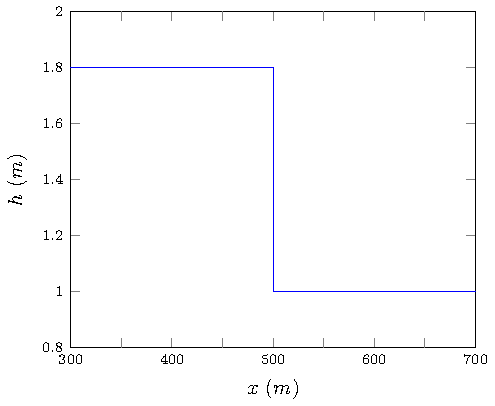
\includegraphics[width=0.75\textwidth]{../Pics/init/DB/DBinit.pdf}
	\end{figure}
\end{frame}

\begin{frame}{Shallow water wave equations analytic solution}
	\begin{figure}
		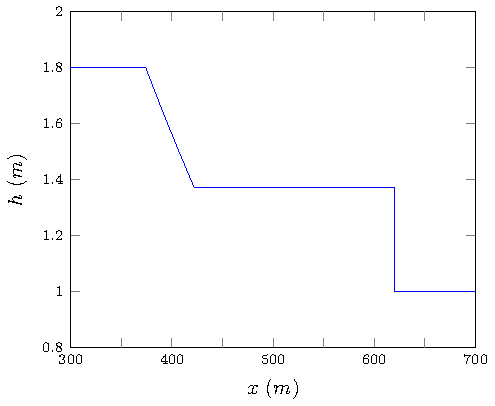
\includegraphics[width=0.75\textwidth]{../Pics/DBana/SWWEana.pdf}
	\end{figure}
\end{frame}

\begin{frame}{Smoothed Dam-Break Problem}
	%Smoothing of dam break
	%Unfortunately some methods in the literature require smooth initial conditions, so we define the smoothed dam-break problem as:
	Solve the Serre equations for $h(x,t)$ and $u(x,t)$ given these initial conditions.
	\begin{subequations}
		\begin{gather*}
		h(x,0) = h_0 + \frac{h_1 - h_0}{2}\left(1 + \tanh\left(\frac{x_0 - x}{\alpha}\right)\right),
		\end{gather*}
		\begin{gather*}
		u(x,0) = 0.0m/s
		\end{gather*}
	\end{subequations}
\end{frame}

\begin{frame}
	Smoothed dam-break for $h_1 = 1.8m$, $h_0 = 1m$ and $x_0 = 500m$
	\begin{figure}
		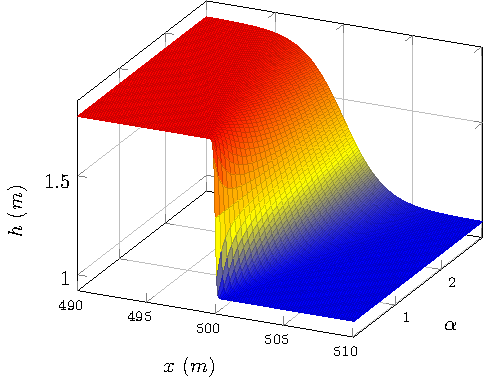
\includegraphics[width=0.75\textwidth]{../Pics/pics/explainers/dbsmooth.pdf}
	\end{figure}
\end{frame}


\begin{frame}{Literature Solutions initial conditions when $\alpha = 0.4m$}
	%Not in literature as alpah too large to approximate dam break problem well
	G. A. El , Roger HJ Grimshaw and Noel F. Smyth (2006)
	\begin{figure}
		\centering
		\begin{subfigure}{0.7\textwidth}
			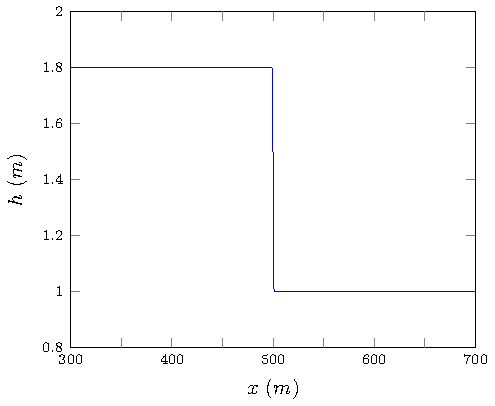
\includegraphics[width=\textwidth]{../Pics/init/DBs9/1-figure0.pdf}
		\end{subfigure}%
	\end{figure}
\end{frame}
\begin{frame}{Literature Solutions $\alpha = 0.4m$}
	G. A. El , Roger HJ Grimshaw and Noel F. Smyth (2006)
	\begin{figure}
		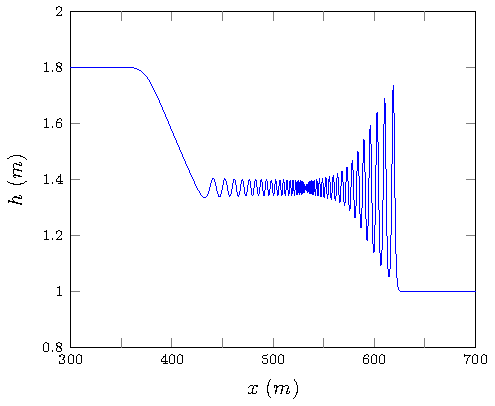
\includegraphics[width=0.7\textwidth]{../Pics/litrec/GrimRec.pdf}
		\label{fig:Litsol2}
	\end{figure}
\end{frame}

\begin{frame}{Literature Solutions initial conditions when $\alpha = 2m$}
	%Not in literature as alpah too large to approximate dam break problem well
	D. Mitsotakis, B. Ilan and D. Dutykh (2014)
	\begin{figure}
		\centering
		\begin{subfigure}{0.7\textwidth}
			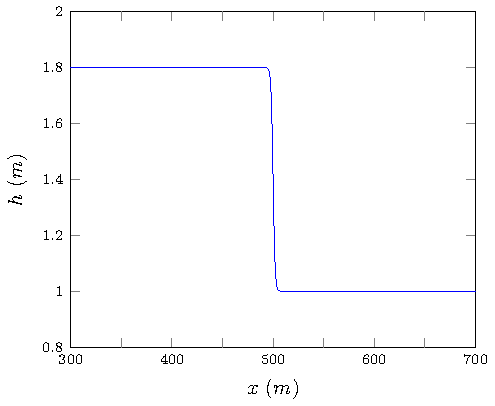
\includegraphics[width=\textwidth]{../Pics/init/DBs6/1-figure0.pdf}
		\end{subfigure}%
	\end{figure}
\end{frame}
\begin{frame} {Literature Solutions $\alpha = 2m$}
	D. Mitsotakis, B. Ilan and D. Dutykh (2014)
	\begin{figure}
		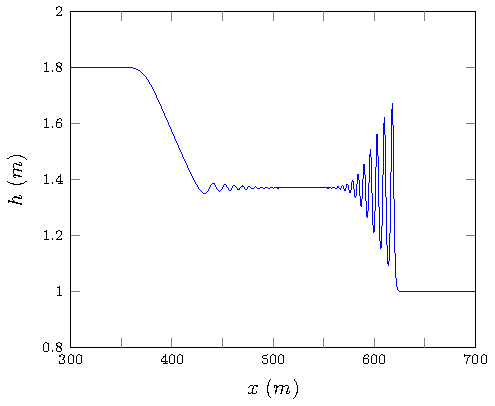
\includegraphics[width=0.7\textwidth]{../Pics/litrec/HankRec.pdf}
	\end{figure}
	%Also supported by later literature results using smoothing of initial conditions
\end{frame}


\begin{frame}{Problem}	
	Goal: numerically model a tsunami throughout its evolution efficiently and robustly.
	\vskip 0.2cm	
	Step 1: We choose the Serre equations 
	\vskip 0.2cm
	Step 2: Presented some efficient methods
	\vskip 0.2cm
	Problem: Check robustness without analytic solutions for Serre equations involving steep gradients
	\vskip 0.2cm
	Attempt: Numerically solve simplest problem with a steep gradient.
	
\end{frame}

\section{Results}
%Careful about the end time, explain this situation
\subsection{Structures}

\begin{frame}{Structures}
	We found 4 different structures for numerical solutions of the Serre equations to various smoothed dam-break problems using our highest order method finite volume method with highest resolution.
	\begin{itemize}
		\item Non-oscillatory structure
		\item Flat structure
		\item Node structure
		\item Growth structure
	\end{itemize}
\end{frame}

%initial conditions

\begin{frame}{Initial conditions when $\alpha = 40m$}
	%Not in literature as alpah too large to approximate dam break problem well
	\begin{figure}
		\centering
		\begin{subfigure}{0.75\textwidth}
			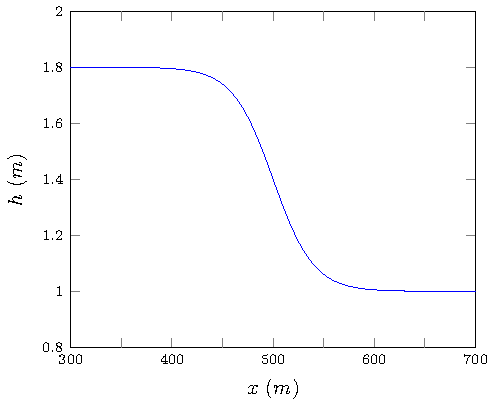
\includegraphics[width=\textwidth]{../Pics/init/DBs1/1-figure0.pdf}
		\end{subfigure}%
	\end{figure}
\end{frame}

\begin{frame}{Non-Oscillatory structure  $\alpha = 40m$}
	%Not in literature as alpah too large to approximate dam break problem well
	\begin{figure}
		\centering
		\begin{subfigure}{0.75\textwidth}
			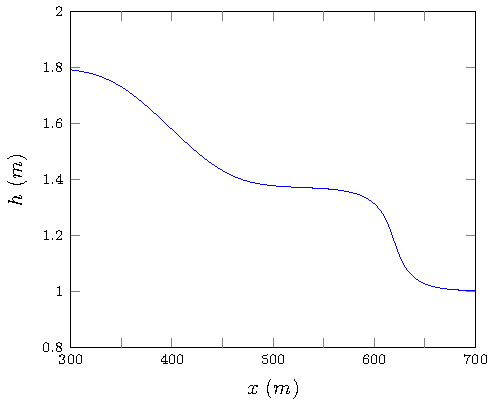
\includegraphics[width=\textwidth]{../Pics/DBstruct/1.pdf}
		\end{subfigure}%
	\end{figure}
\end{frame}

\begin{frame}{Initial conditions when $\alpha = 2m$}
	%Not in literature as alpah too large to approximate dam break problem well
	\begin{figure}
		\centering
		\begin{subfigure}{0.75\textwidth}
			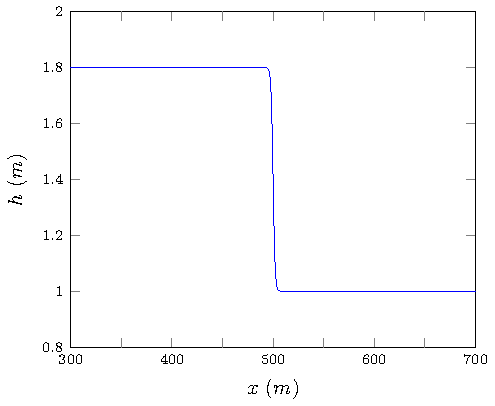
\includegraphics[width=\textwidth]{../Pics/init/DBs6/1-figure0.pdf}
		\end{subfigure}%
	\end{figure}
\end{frame}

\begin{frame}{Flat $\alpha = 2m$}
	%Most common in the literature, using similar alpha values, or using poor methods.
	\begin{figure}
		\begin{subfigure}{0.75\textwidth}
			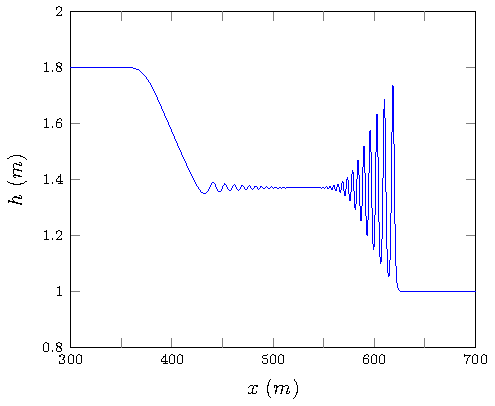
\includegraphics[width=\textwidth]{../Pics/DBstruct/6.pdf}
		\end{subfigure}
	\end{figure}
\end{frame}

\begin{frame}{Initial conditions when $\alpha = 0.4m$}
	%Not in literature as alpah too large to approximate dam break problem well
	\begin{figure}
		\centering
		\begin{subfigure}{0.75\textwidth}
			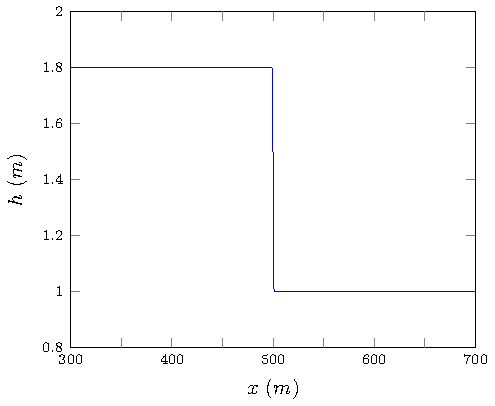
\includegraphics[width=\textwidth]{../Pics/init/DBs9/1-figure0.pdf}
		\end{subfigure}%
	\end{figure}
\end{frame}

\begin{frame}{Node $\alpha = 0.4m$}
	%Grimshaws result
	\begin{figure}
		\begin{subfigure}{0.75\textwidth}
			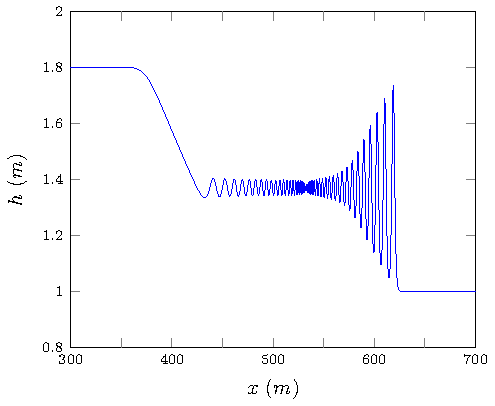
\includegraphics[width=\textwidth]{../Pics/DBstruct/9.pdf}
		\end{subfigure}
	\end{figure}
\end{frame}

\begin{frame}{Initial conditions when $\alpha = 0.1m$}
	%Not in literature as alpah too large to approximate dam break problem well
	\begin{figure}
		\centering
		\begin{subfigure}{0.75\textwidth}
			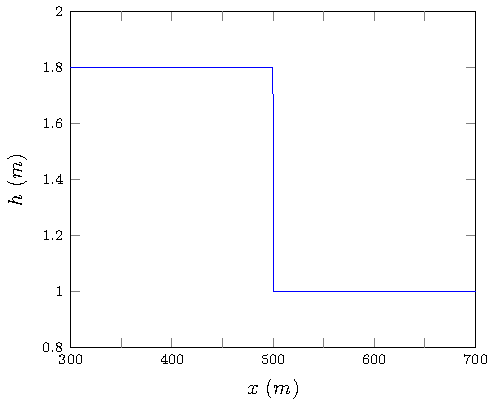
\includegraphics[width=\textwidth]{../Pics/init/DBs12/1-figure0.pdf}
		\end{subfigure}%
	\end{figure}
\end{frame}

\begin{frame}{Growth ($\alpha = 0.1m$)}
	%not commonly published in literature for these equations at least
	%if these results are correct, the Serre equations for the dam-break problem will possess a growth structure
	\begin{figure}
		\begin{subfigure}{0.75\textwidth}
			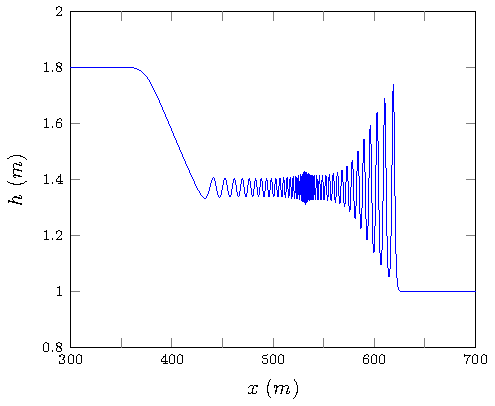
\includegraphics[width=\textwidth]{../Pics/DBstruct/12.pdf}
		\end{subfigure}
	\end{figure}
\end{frame}

\subsection{Verification}

\begin{frame}{Problem}
	
	Goal: numerically model a tsunami throughout its evolution efficiently and robustly.
	\vskip 0.2cm
	Step 1: We choose the Serre equations 
	\vskip 0.2cm
	Step 2: Presented some efficient methods
	\vskip 0.2cm
	Problem: Check robustness without analytic solutions for Serre equations involving steep gradients
	\vskip 0.2cm
	Attempt: Numerically solve simplest problem with a steep gradient.
	\vskip 0.2cm
	New Problem: Are these numerical results correct?	
\end{frame}

\begin{frame}{Growth structure: changing resolutions}
	Although we cannot check if our numerical solutions are converging to a true solution as one is not known for the Serre equations we can check if the numerical solutions converge to one another as $\Delta x \rightarrow 0$. 
	\vskip 0.2cm
	We will now perform this for our highest order finite volume method, with an initial $\Delta x$ of $0.5m$, resolution is increased by dividing $\Delta x$ by $4$.
\end{frame}

\begin{frame}{Initial conditions when $\alpha = 0.1m$}
	%Not in literature as alpah too large to approximate dam break problem well
	\begin{figure}
		\centering
		\begin{subfigure}{0.75\textwidth}
			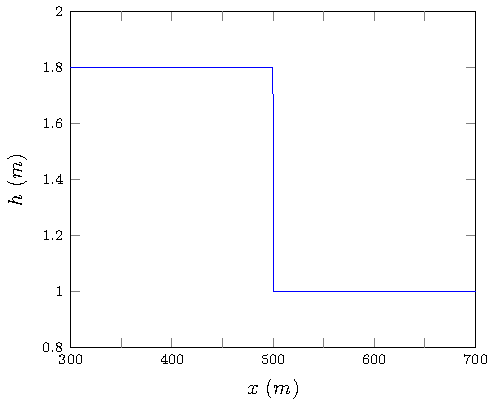
\includegraphics[width=\textwidth]{../Pics/init/DBs12/1-figure0.pdf}
		\end{subfigure}%
	\end{figure}
\end{frame}

\begin{frame}{Growth structure: changing resolutions}
		\begin{figure}
			\begin{subfigure}{0.75\textwidth}
				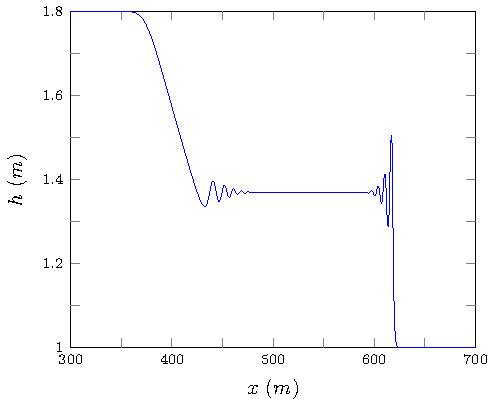
\includegraphics[width=\textwidth]{../Pics/dx0/4/1-figure0.pdf}
			\end{subfigure}
		\end{figure}
\end{frame}

\begin{frame}{Growth structure: changing resolutions}
	\begin{figure}
		\begin{subfigure}{0.75\textwidth}
			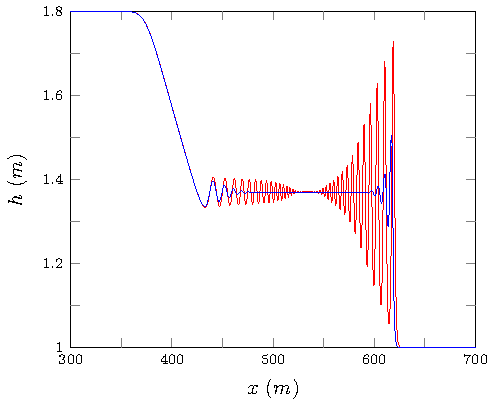
\includegraphics[width=\textwidth]{../Pics/dx0/46/1-figure0.pdf}
		\end{subfigure}
	\end{figure}
\end{frame}

\begin{frame}{Growth structure: changing resolutions}
	\begin{figure}
		\begin{subfigure}{0.75\textwidth}
			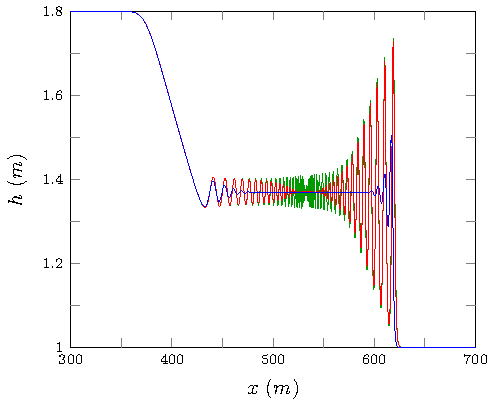
\includegraphics[width=\textwidth]{../Pics/dx0/468/1-figure0.pdf}
		\end{subfigure}
	\end{figure}
\end{frame}

\begin{frame}{Growth structure: changing resolutions}
	\begin{figure}
		\begin{subfigure}{0.75\textwidth}
			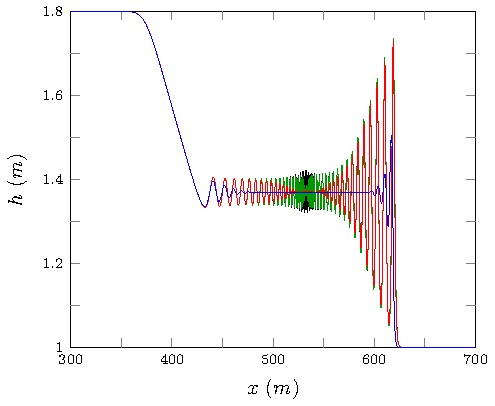
\includegraphics[width=\textwidth]{../Pics/dx0/all/1-figure0.pdf}
		\end{subfigure}
	\end{figure}
\end{frame}

\begin{frame}{Growth structure: changing resolutions}
	\begin{figure}
		\begin{subfigure}{0.75\textwidth}
			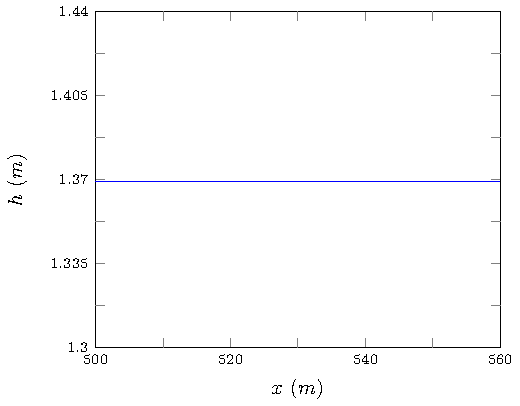
\includegraphics[width=\textwidth]{../Pics/dx0/4/2-figure0.pdf}
		\end{subfigure}
	\end{figure}
\end{frame}

\begin{frame}{Growth structure: changing resolutions}
	\begin{figure}
		\begin{subfigure}{0.75\textwidth}
			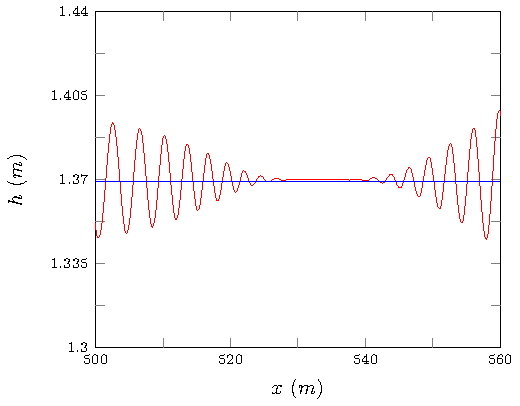
\includegraphics[width=\textwidth]{../Pics/dx0/46/2-figure0.pdf}
		\end{subfigure}
	\end{figure}
\end{frame}

\begin{frame}{Growth structure: changing resolutions}
	\begin{figure}
		\begin{subfigure}{0.75\textwidth}
			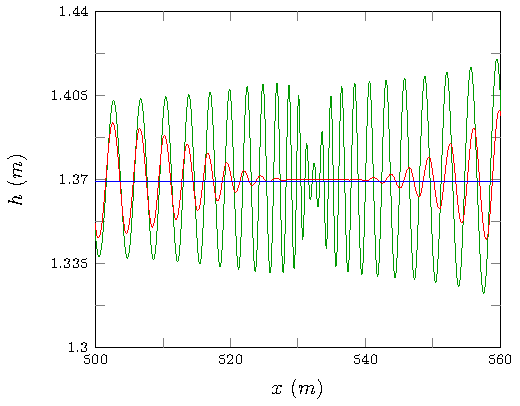
\includegraphics[width=\textwidth]{../Pics/dx0/468/2-figure0.pdf}
		\end{subfigure}
	\end{figure}
\end{frame}

\begin{frame}{Growth structure: changing resolutions}
	\begin{figure}
		\begin{subfigure}{0.75\textwidth}
			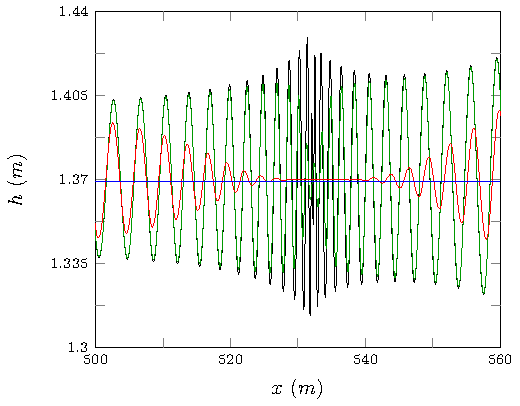
\includegraphics[width=\textwidth]{../Pics/dx0/all/2-figure0.pdf}
		\end{subfigure}
	\end{figure}
\end{frame}

\begin{frame}{Growth structure: changing resolutions}
	\begin{figure}
		\begin{subfigure}{0.75\textwidth}
			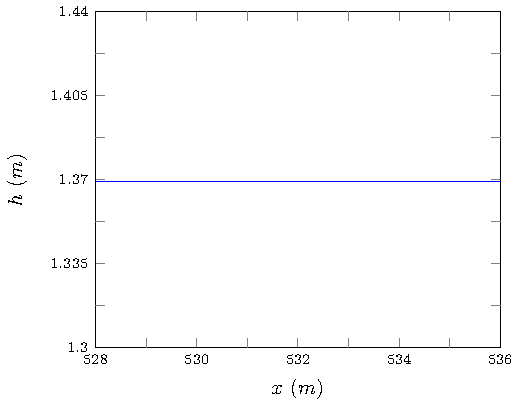
\includegraphics[width=\textwidth]{../Pics/dx0/4/4-figure0.pdf}
		\end{subfigure}
	\end{figure}
\end{frame}

\begin{frame}{Growth structure: changing resolutions}
	\begin{figure}
		\begin{subfigure}{0.75\textwidth}
			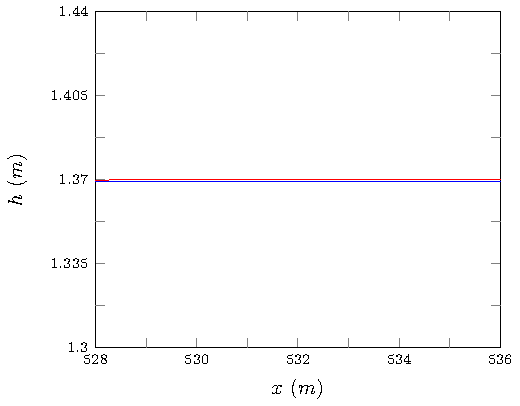
\includegraphics[width=\textwidth]{../Pics/dx0/46/4-figure0.pdf}
		\end{subfigure}
	\end{figure}
\end{frame}

\begin{frame}{Growth structure: changing resolutions}
	\begin{figure}
		\begin{subfigure}{0.75\textwidth}
			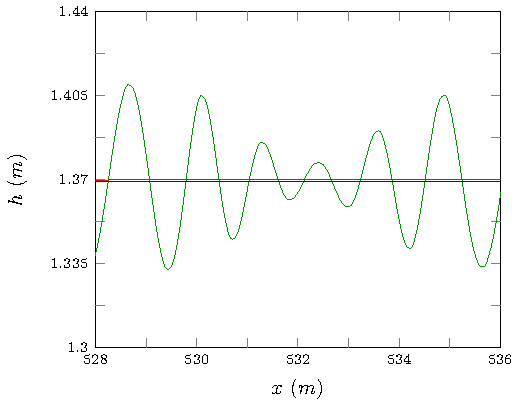
\includegraphics[width=\textwidth]{../Pics/dx0/468/4-figure0.pdf}
		\end{subfigure}
	\end{figure}
\end{frame}

\begin{frame}{Growth structure: changing resolutions}
	\begin{figure}
		\begin{subfigure}{0.75\textwidth}
			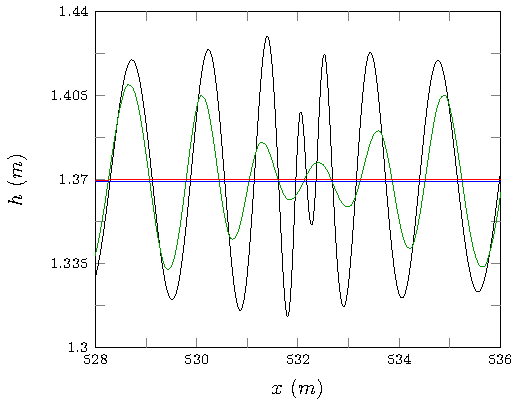
\includegraphics[width=\textwidth]{../Pics/dx0/all/4-figure0.pdf}
		\end{subfigure}
	\end{figure}
\end{frame}

\begin{frame}{Growth structure: conservation while changing resolutions}
	%mention energy
	\begin{table}
		\begin {tabular}{c c c c c}%
		$\alpha$& $\Delta x$&Conservation error ${h}$& Conservation error ${uh}$ \\		
		$0.1$ &$0.2$&\pgfutilensuremath {7.6\cdot 10^{-14}}&\pgfutilensuremath {4.82\cdot 10^{-3}}\\		
		$0.1$ &$0.05$&\pgfutilensuremath {2.4\cdot 10^{-13}}&\pgfutilensuremath {2.39\cdot 10^{-4}}\\		
		$0.1$ &$0.0125$&\pgfutilensuremath {9.79\cdot 10^{-13}}&\pgfutilensuremath {2.21\cdot 10^{-7}}\\		
		$0.1$ &$0.003125$&\pgfutilensuremath {3.92\cdot 10^{-12}}&\pgfutilensuremath {4.46\cdot 10^{-8}}\\
		\end {tabular}%
	\end{table}
	
\end{frame}

\begin{frame}{Growth structure: changing resolutions}
This shows that:
\vskip 0.2cm
1. Away from the growth in oscillations the numerical solutions converge quite well
\vskip 0.2cm
2. Main difference in solutions is amplitude of oscillations (indicating that these are not of numerical origin)
\vskip 0.2cm
3. Our numerical methods are approaching a solution which is conservative

\end{frame}

\begin{frame}{Growth structure: changing methods}
We want our numerical solutions to not be model dependent for high resolution grids and fixed $\alpha$.
\vskip 0.2cm
We compare two models, the highest order finite volume from before, and a finite difference method.
\end{frame}

\begin{frame}{Initial conditions when $\alpha = 0.1m$}
	%Not in literature as alpah too large to approximate dam break problem well
	\begin{figure}
		\centering
		\begin{subfigure}{0.75\textwidth}
			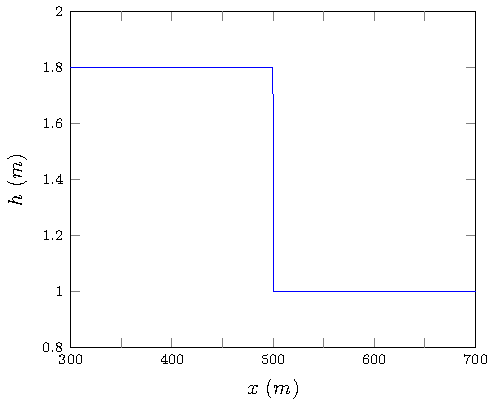
\includegraphics[width=\textwidth]{../Pics/init/DBs12/1-figure0.pdf}
		\end{subfigure}%
	\end{figure}
\end{frame}
\begin{frame}{Growth structure: changing methods}
	\begin{figure}
		\begin{subfigure}{0.75\textwidth}
			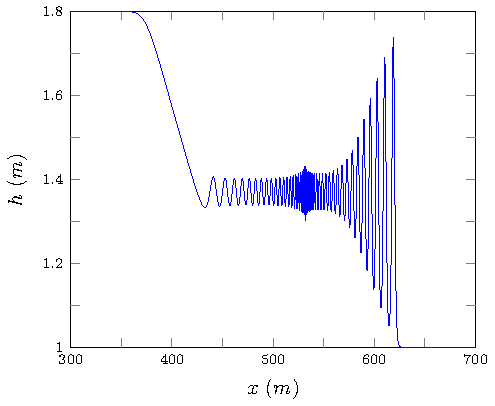
\includegraphics[width=\textwidth]{../Pics/Models/FD/1-figure0.pdf}
		\end{subfigure}
	\end{figure}
\end{frame}

\begin{frame}{Growth structure: changing methods}
	\begin{figure}
		\begin{subfigure}{0.75\textwidth}
			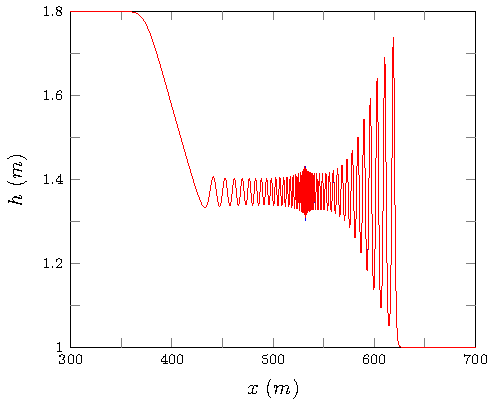
\includegraphics[width=\textwidth]{../Pics/Models/all/1-figure0.pdf}
		\end{subfigure}
	\end{figure}
\end{frame}

\begin{frame}{Growth structure: changing methods}
	\begin{figure}
		\begin{subfigure}{0.75\textwidth}
			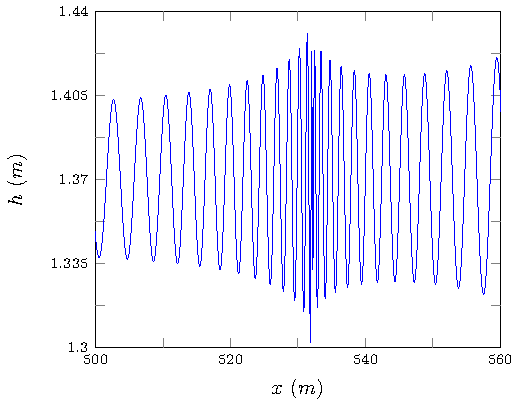
\includegraphics[width=\textwidth]{../Pics/Models/FD/2-figure0.pdf}
		\end{subfigure}
	\end{figure}
\end{frame}

\begin{frame}{Growth structure: changing methods}
	\begin{figure}
		\begin{subfigure}{0.75\textwidth}
			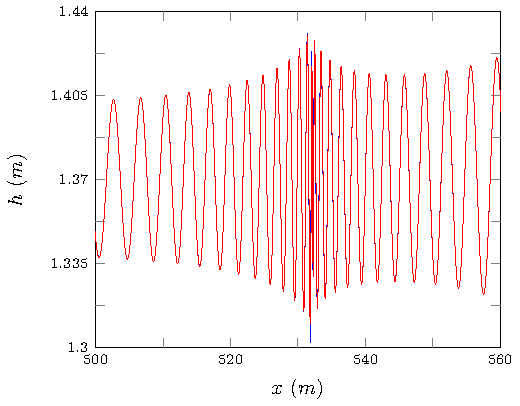
\includegraphics[width=\textwidth]{../Pics/Models/all/2-figure0.pdf}
		\end{subfigure}
	\end{figure}
\end{frame}

\begin{frame}{Growth structure: changing methods}
	\begin{figure}
		\begin{subfigure}{0.75\textwidth}
			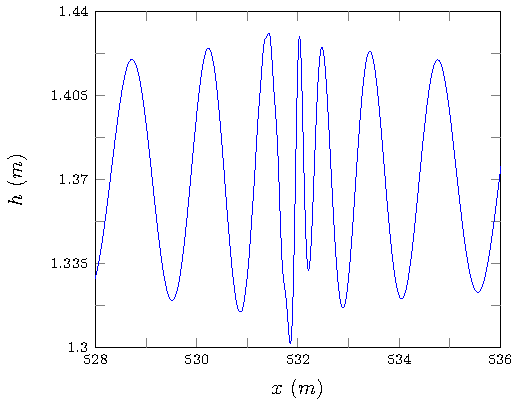
\includegraphics[width=\textwidth]{../Pics/Models/FD/4-figure0.pdf}
		\end{subfigure}
	\end{figure}
\end{frame}

\begin{frame}{Growth structure: changing methods}
	\begin{figure}
		\begin{subfigure}{0.75\textwidth}
			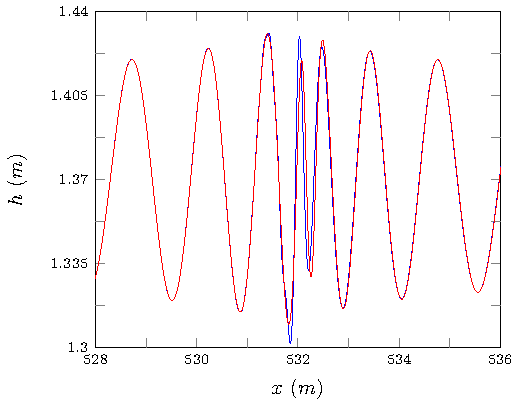
\includegraphics[width=\textwidth]{../Pics/Models/all/4-figure0.pdf}
		\end{subfigure}
	\end{figure}
\end{frame}

\begin{frame}{Growth structure: changing methods}
	This shows that:
	\vskip 0.2cm
	1. Just a very few oscillations are different across the models
	\vskip 0.2cm
	2. Again only difference is amplitude of oscillations
	\vskip 0.2cm
	3. Structure independent of method
	
\end{frame}

\begin{frame}{Growth structure: conclusion}
\begin{itemize}
	\item Numerical solutions for a method converge to one another as $\Delta x \rightarrow 0$
	\item Numerical solutions for a method converge to a conservative solution as $\Delta x \rightarrow 0$
	\item Growth structure is found for different methods
\end{itemize}
	Conclusion: solutions of the Serre equations should exhibit the growth structure for the smoothed dam-break problem with small $\alpha$ and even the dam-break problem. 
\end{frame}

\begin{frame}{Problem}
	
	Goal: numerically model a tsunami throughout its evolution efficiently and robustly.
	\vskip 0.2cm
	Step 1: We choose the Serre equations 
	\vskip 0.2cm
	Step 2: Presented some efficient methods
	\vskip 0.2cm
	Step 3: Numerically solved Serre equations in the presence of steep gradients and verified our solutions.
		
\end{frame}

\begin{frame}{Further Work}
	
	Goal: numerically model a tsunami throughout its evolution efficiently and robustly.
	\vskip 0.2cm
	Sub Goal: Inundation of land, have to solve the dry bed problem for our numerical solutions
	\vskip 0.2cm
	Sub Goal: Full three dimensional flow
	
\end{frame}



\end{document}